% =====================================================================
%  Mapping Natural-Disaster Damage from Satellite Imagery
%  Final report. Every number comes from results/ in the repository.
% =====================================================================
\documentclass[10pt,twocolumn]{article}

\usepackage[T1]{fontenc}
\usepackage[utf8]{inputenc}
\usepackage{lmodern}
\usepackage{microtype}
\usepackage[htt]{hyphenat}      % let \texttt identifiers hyphenate instead of
                                % stretching the line they sit on
\usepackage[a4paper,margin=1.9cm,columnsep=0.75cm]{geometry}
\usepackage{graphicx}
\usepackage{booktabs}
\usepackage{amsmath}
\usepackage{xcolor}
\usepackage{caption}
\usepackage{subcaption}
\usepackage{enumitem}
\usepackage{fancyhdr}
\usepackage[hidelinks]{hyperref}

% ---------------------------------------------------------------- style
\definecolor{accent}{HTML}{1F4E79}

\captionsetup{font=small,labelfont={bf,color=accent},skip=4pt}
\setlength{\parskip}{0pt}
\setlength{\emergencystretch}{3em}
\setlength{\tabcolsep}{4pt}     % default 6pt overflows the column in a 2-col layout
\tolerance=1200

\renewcommand{\topfraction}{0.92}
\renewcommand{\bottomfraction}{0.7}
\renewcommand{\textfraction}{0.07}
\renewcommand{\floatpagefraction}{0.75}
\setcounter{topnumber}{3}
\setcounter{totalnumber}{5}

\pagestyle{fancy}
\fancyhf{}
\renewcommand{\headrulewidth}{0.4pt}
\fancyhead[L]{\footnotesize\color{accent}Mapping Natural-Disaster Damage from Satellite Imagery}
\fancyhead[R]{\footnotesize\color{accent}\thepage}

\newcommand{\class}[1]{\textsf{#1}}

% =====================================================================
\begin{document}

\twocolumn[
\begin{@twocolumnfalse}
\begin{center}

{\LARGE\bfseries Mapping Natural-Disaster Damage from Satellite Imagery\par}
\vspace{3pt}
{\large Cross-disaster transfer on xBD: pretrained versus from-scratch change-detection CNNs\par}

\vspace{8pt}
{\normalsize Artur Zavistovskyi, Bhuvanesh Dinesh Wadhwani, Anastasiia Khitrova, Yitian Zhou\par}
\vspace{2pt}
{\footnotesize Deep Learning Final Project\par}

\vspace{10pt}
\end{center}

\noindent{\small
\textbf{Abstract.} This project addresses two questions about automated building-damage
classification on xBD: whether performance transfers from a set of disaster types seen in training
to a disaster type withheld entirely, and whether ImageNet pretraining improves that transfer
relative to a comparably designed encoder trained from scratch. Two siamese change-detection CNNs
that differ only in the encoder, one an ImageNet-pretrained ResNet-18, one a compact encoder trained
from scratch, are trained on 14 non-fire disaster events under identical patches, splits and class
weights, then evaluated both in-distribution and zero-shot on five wildfire events held out entirely.
The pretrained model reaches 0.808 accuracy and 0.650 macro-F1 in distribution, falling to 0.774
accuracy and 0.429 macro-F1 on wildfire, a 33.9\% relative loss in macro-F1. This aggregate drop
does not indicate a general representation failure: \class{destroyed} scores higher out of
domain than in it (F1 0.758 versus 0.687), \class{no-damage} precision reaches 0.966, and
threshold-free ROC-AUC holds at 0.814. The degradation is confined to the two intermediate damage
classes, which make up 19.1\% of training patches but only 1.7\% of wildfire patches, indicating
that the learned visual features transfer across disaster types while the decision calibration,
tuned to the training-domain class prior, does not. Comparing the two encoders, pretraining
outperforms training from scratch on every split and every metric, with the largest margin precisely
where it matters most: $+0.143$ accuracy and $+0.052$ macro-F1 on the wildfire set. A third analysis
joins 185,045 labelled buildings to census block groups and finds that an apparent association
between median income and damage ($\beta = +0.225$, $p = 0.0009$) disappears once event fixed
effects are added ($\beta = +0.057$, $p = 0.44$): the association is explained by which disaster
struck which place, not by income differences within a disaster. Recovery capacity tells a different
story: pricing the same damage in dollars against HAZUS loss ratios, validated against NFIP, CAL FIRE
and FEMA records, exposes a steep income gradient, with 61\% of the poorest income quartile's flood
loss covered by neither insurance nor federal aid against 34\% in the richest, and auditing the two
Part~2 models' own predictions shows that an automated relief rule would misdirect \$30--78M of every
\$1B on seen disaster types and \$112--200M on wildfire, the type the models never trained on.
\par}
\vspace{9pt}
\end{@twocolumnfalse}
]

% =====================================================================
\section{Introduction}

Automated damage maps are operationally useful only if they generalise to disaster types for which
no labelled data yet exists. In-distribution accuracy does not measure this: a model can perform well
on held-out data drawn from the same disaster types it was trained on while failing on a disaster
type it has never encountered. This report addresses two related questions. First, how much of a
change-detection model's performance transfers when it is evaluated on a disaster type withheld
entirely from training. Second, whether ImageNet pretraining improves that transfer relative to a
comparably designed encoder trained from scratch on the same data, since pretraining is a design
choice available at no additional labelling cost.

We study these questions on xBD~\cite{xbd}, the dataset behind the xView2 challenge~\cite{xview2},
which pairs pre- and post-event high-resolution satellite tiles with building footprints and a
four-level damage scale. Prior work on this data fuses the two time steps inside the network
\cite{fusion}; we instead keep the comparison explicit in the classification head, for the reason
given in Section~\ref{sec:arch}. The task is framed as change detection at building level:
given two co-registered crops of the same structure, one before and one after the event, predict
\class{no-damage}, \class{minor-damage}, \class{major-damage} or \class{destroyed}.

The experimental design avoids a random split. Five wildfire events are withheld from training
entirely and used as a zero-shot test set, while the official xView2 evaluation directories provide
an in-distribution reference measured on the same trained model. Both encoders, pretrained and
from-scratch, are evaluated identically on both sets, so the results address the transfer question
and the pretraining question together rather than in isolation.

\section{Data}

\subsection{Source and access}

We use the full xBD release: 11,034 scenes over 19 events, each contributing a $1024\times1024$ RGB
pre-disaster tile, the matching post-disaster tile, and a GeoJSON label file. That is 22,068 images
and 425,368 annotated building polygons on the post-disaster side, obtained through a
public mirror of the xView2 challenge release.\footnote{Kaggle dataset
\texttt{qianlanzz/\allowbreak xbd-dataset}, layout
\texttt{xbd/\{hold,\allowbreak test,\allowbreak tier1,\allowbreak tier3\}/\allowbreak \{images,\allowbreak labels\}}.}

Two properties of the source were verified rather than assumed. First, the tiles are
co-registered: pixel $(x,y)$ denotes the same ground location before and after the event, which is
what makes cropping an identical bounding box from both tiles valid; without this property the
siamese design would be comparing different places. Second, the format is uniform: all 800
files in a stratified quality-control sample decode as $1024\times1024$ RGB PNG with no read errors,
so no resolution standardisation or band alignment is required. Damage labels are recorded only in
the post-disaster GeoJSON, under
\texttt{features.xy[].\allowbreak properties.\allowbreak subtype}; the same file carries \texttt{features.\allowbreak lng\_lat}, giving
per-building WGS84 coordinates, so the geo-referencing for Part 3 is already present.

\subsection{Split design}

The split is scene-level and was produced by a dedicated indexing script rather than inside a
training notebook, so every model in the project trains on an identical partition
(Table~\ref{tab:splits}).

Two aspects of the split design merit comment. First, \texttt{test\_id} is drawn from the official
\texttt{test} and \texttt{hold} directories, which were never part of any training pool and, unlike
\texttt{val}, were never used for tuning, so they provide an honest reference for the headline
number. Second, assignment happens at scene level, which guarantees that the pre- and
post-disaster image of a location cannot separate and that no building can appear in two splits.

\begin{table}[t]
\centering
\footnotesize
\caption{Split design and sizes. Only \texttt{train}/\texttt{val} depend on the random seed; both
test sets are defined by the data itself.}
\label{tab:splits}
\begin{tabular}{@{}llrr@{}}
\toprule
\textbf{Split} & \textbf{Rule} & \textbf{Scenes} & \textbf{Polygons} \\
\midrule
\texttt{train}     & tier1+3, non-fire   & 3,135 & 225,506 \\
\texttt{val}       & tier1+3, non-fire   &   392 &  30,794 \\
\texttt{test\_id}  & test+hold, non-fire & 1,135 &  91,755 \\
\texttt{test\_ood} & wildfire, all       & 6,372 &  77,313 \\
\midrule
\multicolumn{2}{@{}l}{Total}             & 11,034 & 425,368 \\
\bottomrule
\end{tabular}
\end{table}

The five held-out events are \texttt{pinery-bushfire}, \texttt{portugal-\allowbreak wildfire},
\texttt{santa-\allowbreak rosa-wildfire}, \texttt{socal-fire} and \texttt{woolsey-fire}. An automated check
confirms zero wildfire scenes in \texttt{train} or \texttt{val}, and zero event overlap between the
training pool and \texttt{test\_ood}.

% =====================================================================
\section{Exploratory analysis}

\subsection{Class imbalance is severe and split-dependent}

\class{no-damage} accounts for 72.0\% of training polygons and the rarest class is $11.6\times$
smaller (Fig.~\ref{fig:classdist}). More importantly the composition is not stable across splits:
\texttt{test\_ood} is 80.2 / 0.9 / 0.9 / 14.7\% against 72.0 / 9.7 / 8.4 / 6.2\% in \texttt{train}.

Plain accuracy is therefore a poor decision metric: always predicting \class{no-damage} scores 0.72
on the training distribution while producing a damage map that never flags damage. We report macro-F1 and
per-class precision and recall as the decision metrics, use inverse-frequency class weights computed
on \texttt{train} only ($0.330 / 2.379 / 2.910 / 4.919$), and key checkpointing and early stopping on
validation macro-F1. Weighting was preferred to resampling: oversampling would repeat the same few
destroyed buildings many times per epoch and invite memorisation, while undersampling would discard
most of the majority signal.

\begin{figure*}[t]
\centering
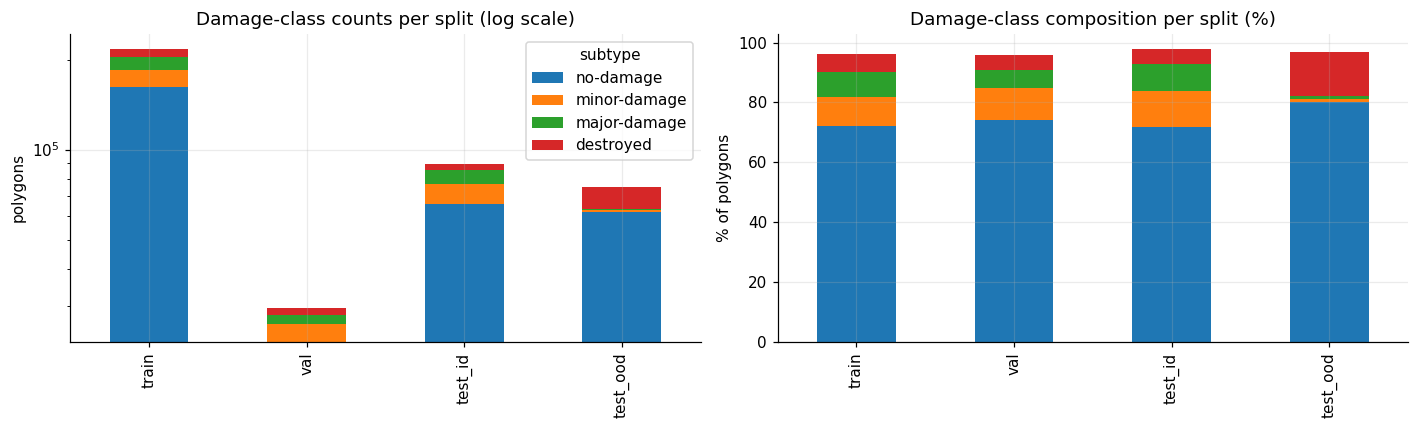
\includegraphics[width=0.85\textwidth]{figures/class_dist_split.png}
\caption{Damage-class distribution per split. Left: counts on a log scale. Right: composition in per
cent. The \texttt{test\_ood} bar is qualitatively different from the other three, with the
intermediate classes almost vanishing and \class{destroyed} more than doubling.}
\label{fig:classdist}
\end{figure*}

\subsection{Wildfire damage is bimodal}

Averaged over events, the non-fire domain is 70.2 / 9.9 / 7.2 / 6.5\% across the four classes while
the wildfire domain is 78.8 / 1.2 / 1.1 / 14.8\%. Fire either leaves a
building intact or destroys it; intermediate states barely occur. Figure~\ref{fig:heatmap} shows
this per event, and also how much the non-fire events differ among themselves:
\texttt{mexico-\allowbreak earthquake} is 99\% undamaged, \texttt{hurricane-\allowbreak matthew} is 51\%
\class{minor-damage}, \texttt{hurricane-\allowbreak harvey} is 35\% \class{major-damage}.

\begin{figure}[t]
\centering
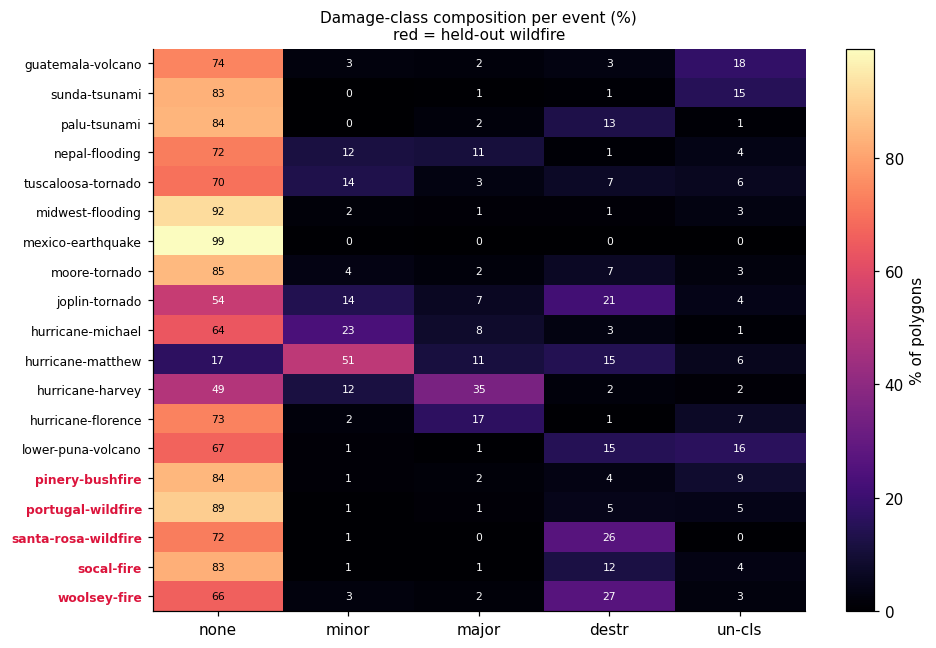
\includegraphics[width=\columnwidth]{figures/class_dist_event.png}
\caption{Damage-class composition per event, in per cent of that event's polygons. Held-out wildfire
events in red. The fire rows share a signature that no non-fire event reproduces: near-zero
\class{minor}/\class{major} with elevated \class{destroyed}.}
\label{fig:heatmap}
\end{figure}

This bimodality operationalises the project's central hypothesis: a model that implicitly learns the
class prior of the non-fire training events will be miscalibrated on fire even if its visual features
transfer perfectly. It also specifies what to look for in the out-of-domain predictions: a pure prior
shift should produce errors with a consistent direction, whereas a failure of the learned features
should produce diffuse, undirected errors.

\subsection{Scene occupancy and patch size}

Empty scenes are common and strongly event-dependent (Fig.~\ref{fig:occupancy}): 9.8\% of training
scenes contain no buildings, against 54.1\% of wildfire scenes, whose median building count
is zero, because the tier3 fire events cover large stretches of forest and scrubland. An empty scene
yields no samples but still costs a full $1024\times1024$ decode, so we sample only scenes with at
least five usable buildings. This is a sampling decision, not a cleaning one: nothing is
deleted, and the identical rule applies to all four splits so it cannot tilt the comparison.

Buildings are small in absolute pixels: the median longest bounding-box side is 35 px and the 90th
percentile 64 px, with a thin tail to 349 px at the 99th. A $64\times64$ patch therefore covers
roughly 90\% of footprints at close to native resolution; larger mostly upsamples empty ground at
quadratic cost, smaller destroys the roof texture separating \class{minor} from \class{major} damage.
We keep a 10 px margin around each footprint, leaving a $44\times44$ px window for the building.
Damage is often more visible around a building than on it (debris, scorch marks, standing
water), but the margin is kept modest deliberately, for reasons Section~\ref{sec:discussion} makes
concrete.

\begin{figure*}[t]
\centering
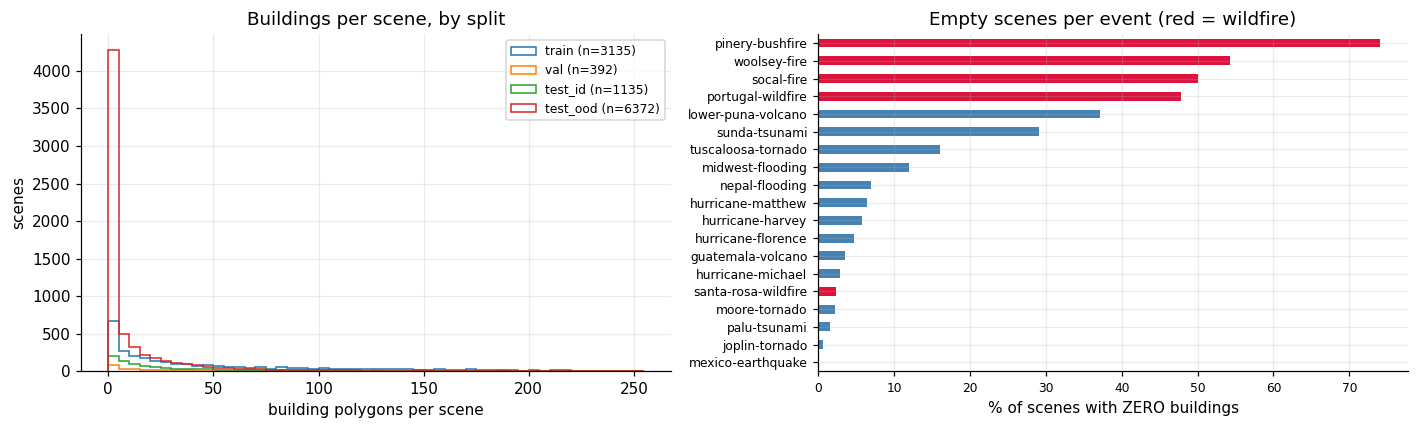
\includegraphics[width=0.85\textwidth]{figures/buildings_per_scene.png}
\caption{Left: distribution of building count per scene by split. Right: share of scenes with zero
buildings, per event (wildfire in red). Four of the five wildfire events are close to or above half
empty; pooled over all wildfire scenes the figure is 54.1\%.}
\label{fig:occupancy}
\end{figure*}

\subsection{A confound in the acquisition geometry}

Ground sample distance and off-nadir angle are similar across the two domains
($2.21 \pm 0.52$ against $2.12 \pm 0.31$ m, and $28.5 \pm 9.9$ against $25.6 \pm 6.0$ degrees), but
sun elevation is not: $64.4 \pm 7.5$ degrees for non-fire against $55.0 \pm 15.9$ for wildfire, with
a fire mode near $35^\circ$ that has no counterpart in training. Low sun means long shadows and a
materially different appearance for the same structure.

\paragraph{Limitation: confounded acquisition geometry.} These spreads overstate their own precision,
because every scene within an event shares a single acquisition. Statistically the effective sample
size is 19 events, not 11,034 scenes, and acquisition geometry is fully confounded with event
identity: wildfire and the specific captures that happen to be wildfire cannot be separated on this
data. Part of the transfer gap reported below may therefore be attributable to shadow length rather
than to fire damage itself, and we cannot bound how much.

\subsection{What the classes look like}

Figure~\ref{fig:examples} contrasts the two domains directly. In the non-fire domain the
post-disaster image usually retains the structure with altered geometry: torn roofs, debris,
standing water. Wildfire damage instead collapses a building to a uniform grey scar with the
footprint faintly visible, while undamaged buildings often sit in surroundings that changed
completely (scorched vegetation) with the roof untouched.

That last observation generates a falsifiable prediction, made before any model was trained: a
change-detection model learns ``the scene changed'' $\Rightarrow$ ``the building is damaged'', so
under wildfire it should over-flag \class{no-damage}. Section~\ref{sec:results} reports the outcome.

\begin{figure*}[t]
\centering
\begin{subfigure}{0.46\textwidth}
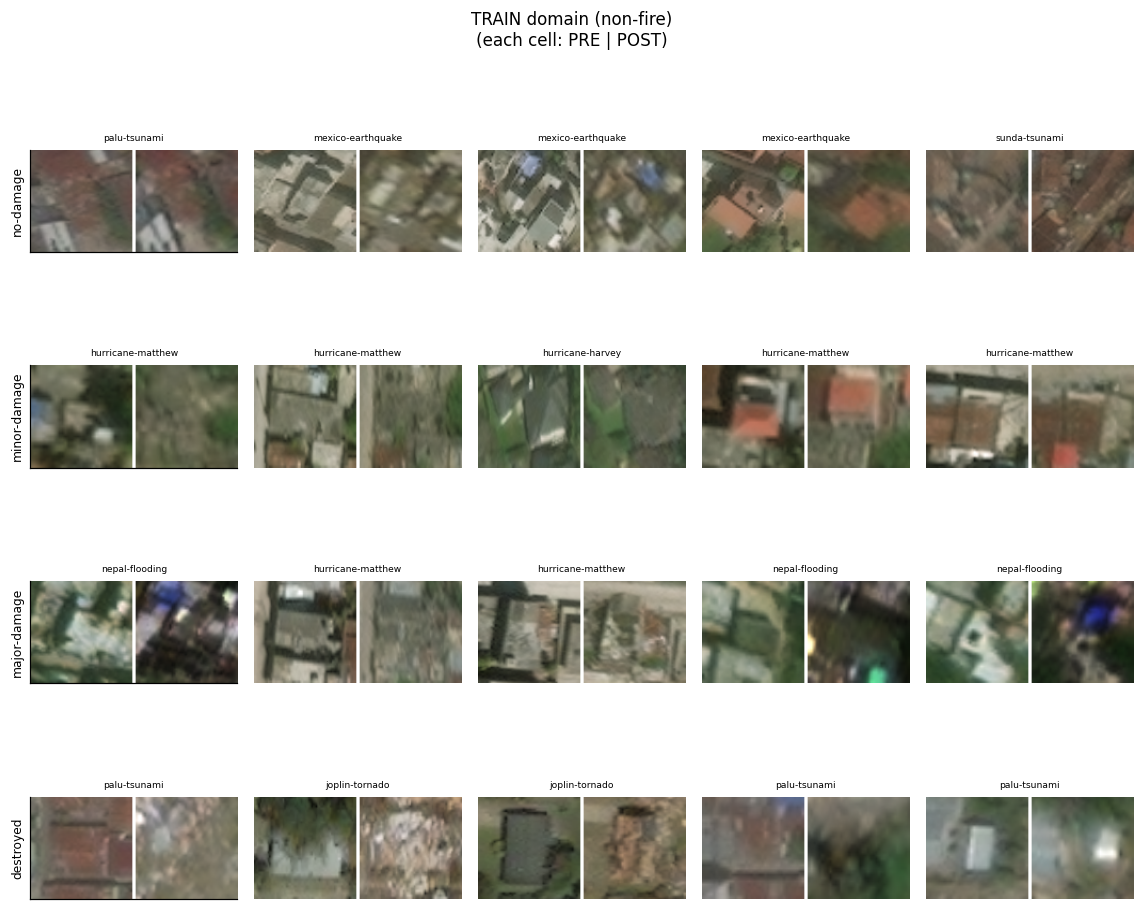
\includegraphics[width=\textwidth]{figures/examples_train.png}
\caption{Training domain (non-fire).}
\end{subfigure}\hfill
\begin{subfigure}{0.46\textwidth}
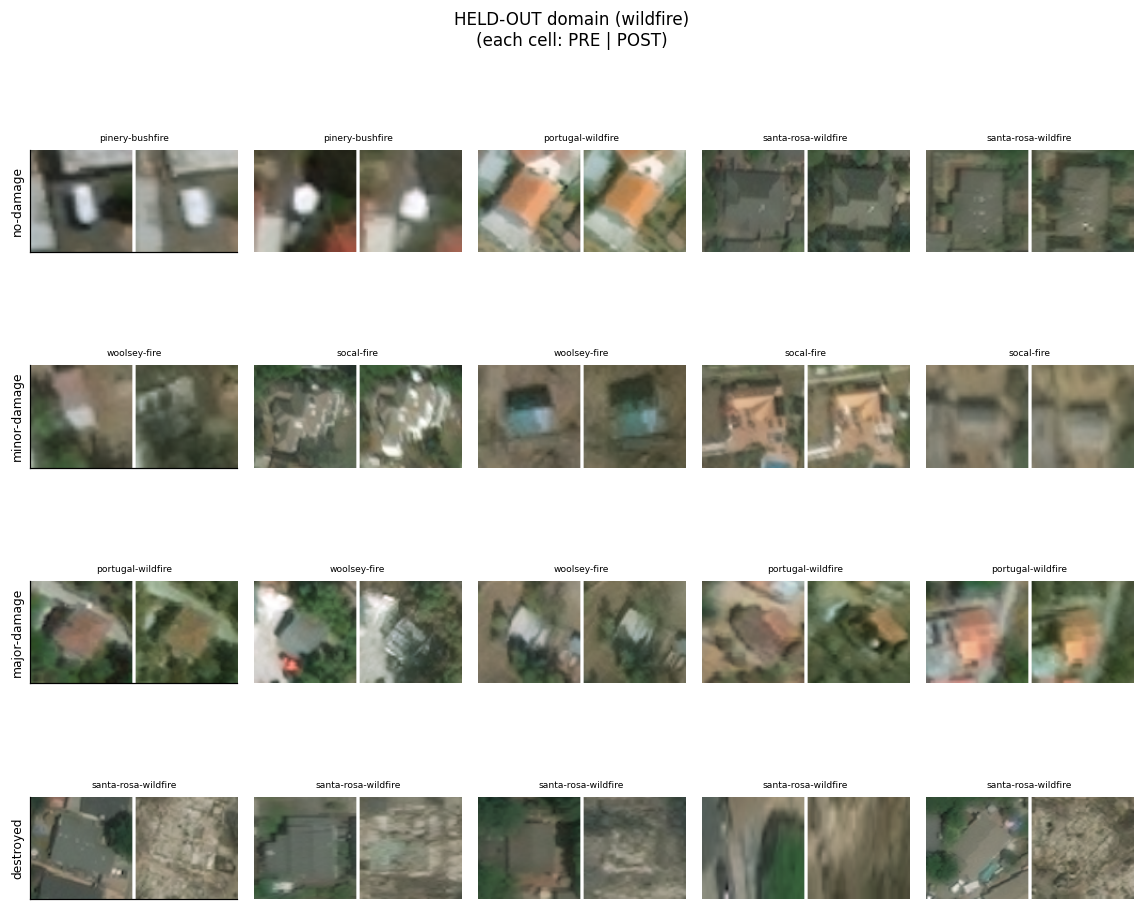
\includegraphics[width=\textwidth]{figures/examples_ood.png}
\caption{Held-out domain (wildfire).}
\end{subfigure}
\caption{Representative building patches, one row per damage class. Each cell shows the pre-disaster
crop on the left and the post-disaster crop on the right.}
\label{fig:examples}
\end{figure*}

% =====================================================================
\section{Data cleaning}

Nothing is removed silently. Every rule states its threshold, its cost and its per-split removal
rate, so a rule that quietly favours one split can be caught. Table~\ref{tab:cleaning} is the ledger.

\begin{table}[t]
\centering
\footnotesize
\caption{Cleaning ledger. Removal is reported against the scope each rule operates on. The 14
occlusion scenes and the 28 near-duplicate pairs were flagged for inspection, not deleted.}
\label{tab:cleaning}
\begin{tabular}{@{}llr@{}}
\toprule
\textbf{Rule} & \textbf{Scope} & \textbf{Removed} \\
\midrule
Missing / unpaired      & 11,034 scenes  & 0 \\
Corrupted images        & 800 files      & 0 \\
Unreadable labels       & 11,034 scenes  & 0 \\
Smoke / cloud           & 683 scenes     & 0 \\
\class{un-classified}   & 425,368 polys  & 14,011 \\
Degenerate polygons     & 425,368 polys  & 0 \\
Side $<8$ px            & 411,357 polys  & 14,458 \\
Near-duplicates         & 400 scenes     & 0 \\
\midrule
\multicolumn{2}{@{}l}{\textbf{Usable after cleaning}}    & \textbf{396,899} \\
\multicolumn{2}{@{}l}{\textbf{(93.3\% of 425,368)}}      & \\
\bottomrule
\end{tabular}
\end{table}

The two rules that cost data are the \class{un-classified} subtype (3.29\% of all polygons) and
sub-8-pixel footprints (3.51\% of the labelled remainder). Both were checked per split. The
\class{un-classified} rate is 3.67 / 4.08 / 2.09 / 3.30\% across
train / val / test\_id / test\_ood, and the tiny-footprint rate is 3.77 / 3.30 / 2.99 / 3.49\%.
Neither is concentrated in \texttt{test\_ood}, so neither flatters the transfer result.

\subsection{The occlusion question: a negative result}

An open data-quality question for this project was whether images obscured by smoke should be
removed. xBD carries no occlusion label: the metadata block contains only capture geometry. The
closest available proxy is the \class{un-classified} subtype, which annotators used when a building
could not be assessed.

The occlusion proxy (the \texttt{un-classified} subtype) was
tested against four whole-tile statistics chosen because
smoke and thin cloud are typically bright, low-contrast,
low-saturation and edge-poor, using a 505-tile sample
enriched toward high-un-classified scenes. Only edge density
showed meaningful correlation (Spearman $-0.366$, explaining
roughly 13\% of the rank variance); brightness, saturation
and contrast were negligible. Flagging the top 2\% of a
composite occlusion score returned 14 scenes ---13
\texttt{sunda-tsunami} and 1 \texttt{lower-puna-volcano}---
none from either test split, so nothing was removed: no
signal was strong enough to justify a threshold, and none of
the flagged scenes touched a reported metric.

\subsection{Leakage checks}

A perceptual-hash duplicate test over the 400-scene
quality-control sample returned 28 near-duplicate pairs,
19 crossing a split boundary. Every cross-split pair
traces back to a handful of low-texture tiles (open
water, unbroken forest, solid cloud) that collide across
unrelated events on different continents ---a single
wildfire tile pairwise identical to tiles from three
other disasters is not plausible as genuine overlap. The
cause is hash degeneracy: a 64-bit difference hash of a
low-texture tile collapses toward a constant, so flat
tiles collide regardless of content. We find no evidence
of leakage, consistent with the scene-level split design.

% =====================================================================
\section{Method}

\subsection{Patch construction}

One sample is two $64\times64\times3$ \texttt{uint8} patches cropped from the same pixel
bounding box in the pre- and post-disaster tile, plus one integer label. Because the tiles are
already co-registered no warping is required; preprocessing is crop, resize, scale to $[0,1]$ and
ImageNet normalisation. Augmentation (flips, 90-degree rotations, brightness jitter) is applied
identically to both images of a pair, since independent jitter per branch would manufacture a
difference where none exists, which is precisely the signal the model is meant to measure.

Scenes were sampled under a compute budget, stratified by event and restricted to scenes with at
least five usable buildings, yielding 135,262 patch pairs from 1,698 scenes
(Table~\ref{tab:patches}). Patches are written to memory-mapped arrays rather than individual image
files, which keeps the working set on disk and the loader fast.

\begin{table}[t]
\centering
\footnotesize
\caption{Extracted patch pairs per split and class. Note the support for \class{minor} and
\class{major} in \texttt{test\_ood}: every per-class number we report for those two classes rests on
these counts.}
\label{tab:patches}
\begin{tabular}{@{}lrrrrr@{}}
\toprule
& \class{none} & \class{minor} & \class{major} & \class{destr} & \textbf{total} \\
\midrule
\texttt{train}     & 55,284 & 7,661 & 6,265 & 3,706 & 72,916 \\
\texttt{val}       & 15,701 & 2,571 & 1,164 & 1,010 & 20,446 \\
\texttt{test\_id}  & 20,500 & 2,840 & 2,512 & 1,421 & 27,273 \\
\texttt{test\_ood} & 12,056 & \textbf{116} & \textbf{138} & 2,317 & 14,627 \\
\midrule
\textbf{Total}     & & & & & \textbf{135,262} \\
\bottomrule
\end{tabular}
\end{table}

\subsection{Architecture}
\label{sec:arch}

The task is a comparison, not the classification of a single image. Using only the post-disaster
patch discards the reference, while stacking pre and post into a six-channel input forces the first
convolution to be relearned, throwing away the pretrained weights exactly where they transfer best.
Both models therefore use a siamese encoder with shared weights and a small head reading
\[
\big[\;f_{\text{pre}},\;\; f_{\text{post}},\;\; \lvert f_{\text{pre}} - f_{\text{post}}\rvert\;\big].
\]
The absolute difference is the explicit change signal; keeping the raw features alongside it lets the
head use appearance as well. Shared weights halve the parameter count and force both branches into a
common feature space, which is what makes the difference term meaningful.

\paragraph{Model A (pretrained).} Uses an ImageNet-pretrained ResNet-18~\cite{resnet,imagenet} encoder,
11.57M parameters in total. At a $64\times64$ input, depth stops paying: architectures designed for
224 px inputs downsample away the little spatial resolution available, and a vision transformer would
reduce a 64 px image to a handful of tokens without the data to compensate for the missing
convolutional prior. ResNet-18 also keeps the comparison honest, since a much larger backbone would
make any win attributable to size rather than pretraining.

\paragraph{Model B (from scratch).} Replaces that encoder with a compact stack built for this problem:
four blocks of two $3\times3$ convolutions with BatchNorm and ReLU followed by $2\times2$
max-pooling, at channel widths $32 \to 64 \to 128 \to 256$, then global average pooling. Total 1.37M
parameters. Everything downstream of the encoder is identical.

\subsection{Training}

Model A follows a linear-probe-then-fine-tune schedule~\cite{lpft}: phase 1 trains only the head on a
frozen backbone for 5 epochs at $10^{-3}$, so the randomly initialised head does not push large
gradients into good weights; phase 2 unfreezes \texttt{layer3} and \texttt{layer4} for up to 45
further epochs at $10^{-4}$, since early layers transfer essentially unchanged while the late
semantic layers must be repurposed. Model B has no pretrained weights to protect, so the whole
network trains from step one at $10^{-3}$ over the same 50-epoch budget.

Both use AdamW with cosine annealing, weight decay $10^{-4}$, weighted cross-entropy with the class
weights above, batch size 128, mixed precision, seed 42, early stopping on validation macro-F1 with
patience 8, and checkpointing on the same criterion. Both are implemented in
PyTorch~\cite{pytorch} and ran locally on an NVIDIA RTX 5070
Laptop GPU; Model A stopped after 43 epochs with the best checkpoint at epoch 35; Model B stopped
after 16 epochs with the best checkpoint at epoch 8, in 14.2 minutes at 53 s per epoch.

\begin{figure}[t]
\centering
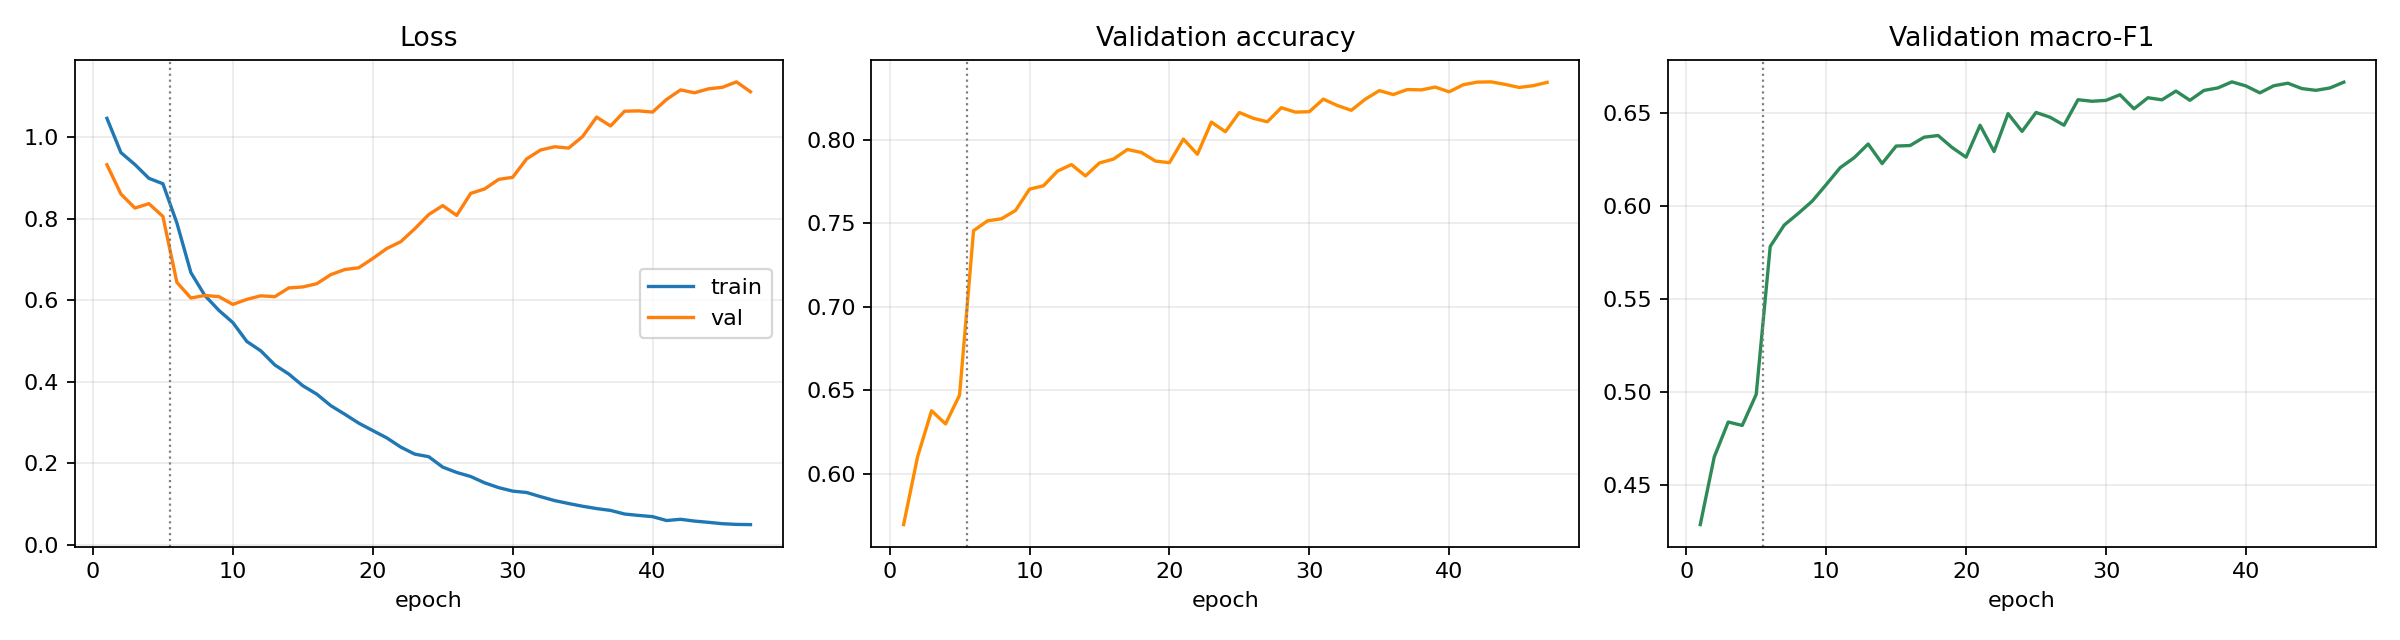
\includegraphics[width=\columnwidth]{figures/training_curves.png}
\caption{Model A training history. Validation loss bottoms out at epoch 11 and then rises steadily,
while validation macro-F1 keeps improving to epoch 35. Model B shows the same pattern.}
\label{fig:curves}
\end{figure}

Two observations from the curves (Fig.~\ref{fig:curves}) are worth recording. Unfreezing lifted Model
A's validation macro-F1 from 0.499 to 0.580 in a single epoch, the clearest evidence here
that a frozen ImageNet backbone is not sufficient for satellite imagery. From its epoch-11 minimum
(0.588), Model A's validation loss then climbs to 1.027 by the best checkpoint and 1.130 by
the end, while macro-F1 improves over the same stretch (0.633 to 0.666). Under a weighted loss on
imbalanced data this is expected, since the model grows over-confident faster than it grows wrong,
and it is why loss would have been the wrong early-stopping criterion. The same decoupling appears in
Model B, on a differently initialised network with a different schedule, so it is a property of the
objective rather than of one run.

% =====================================================================
\section{Results}
\label{sec:results}

\begin{table}[t]
\centering
\footnotesize
\caption{Headline results. Two trained models, three evaluation sets each. P is the pretrained
ResNet-18 encoder, S the from-scratch encoder. \texttt{val} and \texttt{test\_id} are seen disaster
types, \texttt{test\_ood} is the held-out wildfire set; the drops are \texttt{test\_id} to
\texttt{test\_ood}.}
\label{tab:main}
\begin{tabular}{@{}llrrr@{}}
\toprule
\textbf{Split} & & \textbf{Acc.} & \textbf{Macro-F1} & \textbf{AUC} \\
\midrule
\texttt{val}       & P & \textbf{0.830} & \textbf{0.666} & \textbf{0.910} \\
                   & S & 0.763 & 0.597 & 0.902 \\
\texttt{test\_id}  & P & \textbf{0.808} & \textbf{0.650} & \textbf{0.908} \\
                   & S & 0.768 & 0.615 & 0.903 \\
\texttt{test\_ood} & P & \textbf{0.774} & \textbf{0.429} & \textbf{0.814} \\
                   & S & 0.630 & 0.377 & 0.790 \\
\midrule
Abs. drop          & P & $-0.034$  & $-0.221$  & $-0.094$ \\
                   & S & $-0.138$  & $-0.238$  & $-0.113$ \\
Rel. drop          & P & $-4.2\%$  & $-33.9\%$ & $-10.4\%$ \\
                   & S & $-17.9\%$ & $-38.7\%$ & $-12.5\%$ \\
\bottomrule
\end{tabular}
\end{table}

Table~\ref{tab:main} gives the headline numbers. For both models \texttt{val} and \texttt{test\_id}
agree closely (0.666 against 0.650 macro-F1 for P, 0.597 against 0.615 for S), which matters: it
shows the in-distribution figure is not a lucky validation draw, so the \texttt{test\_ood} gap is a
genuine domain effect rather than noise.

\subsection{Per-class behaviour}

The aggregate drop is misleading, and the per-class view (Fig.~\ref{fig:perclass}) shows why.

\begin{figure*}[t]
\centering
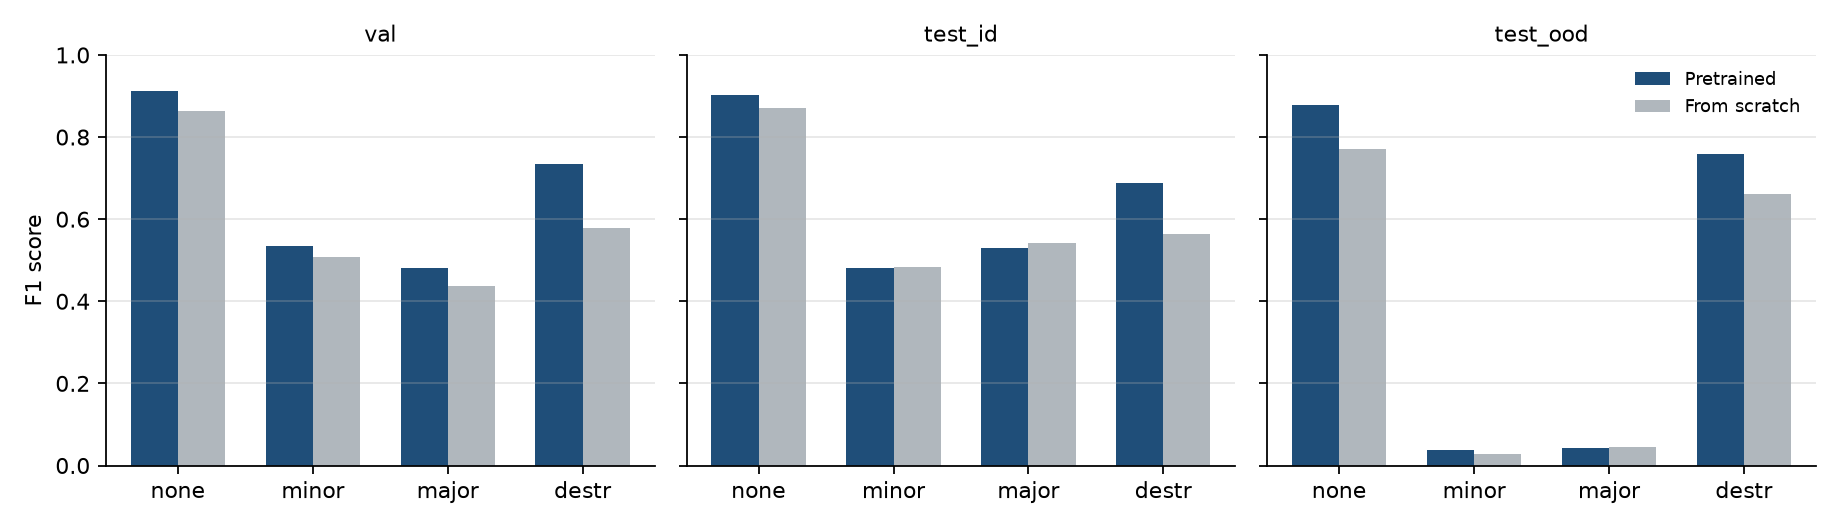
\includegraphics[width=0.85\textwidth]{figures/per_class_f1.png}
\caption{Per-class F1 for both models on the three evaluation sets. In domain the two are close on
the intermediate classes and pretraining mostly buys \class{destroyed}; out of domain both collapse
on \class{minor} and \class{major}, and the pretrained advantage on \class{destroyed} widens.}
\label{fig:perclass}
\end{figure*}

For the pretrained model, \class{destroyed} scores F1 0.758 on wildfire against 0.687 in domain, at
precision 0.872, and \class{no-damage} reaches precision 0.966. Despite never having been trained on
wildfire imagery, the model identifies destroyed buildings under wildfire more reliably than it
identifies destroyed buildings from the disaster types it was trained on. The degradation is confined
entirely to the two intermediate classes, whose F1 falls from 0.480 and 0.529 in domain to 0.038 and
0.043 on wildfire. What breaks is precision, down to 0.020 and 0.024; recall does not vanish
(0.284 and 0.203).

\subsection{Error structure}

The over-prediction is systematic rather than isolated. Against 116 true \class{minor} and 138 true
\class{major} patches, the pretrained model emits 2,814 intermediate predictions and the
from-scratch model 4,713, an over-prediction of $11.1\times$ and $18.6\times$. That alone caps
combined precision near 0.02 regardless of how good the features are. Figure~\ref{fig:predictions}
shows a concrete instance of the pretrained model's failure mode alongside a correct prediction from
each test split.

\begin{figure}[t]
\centering
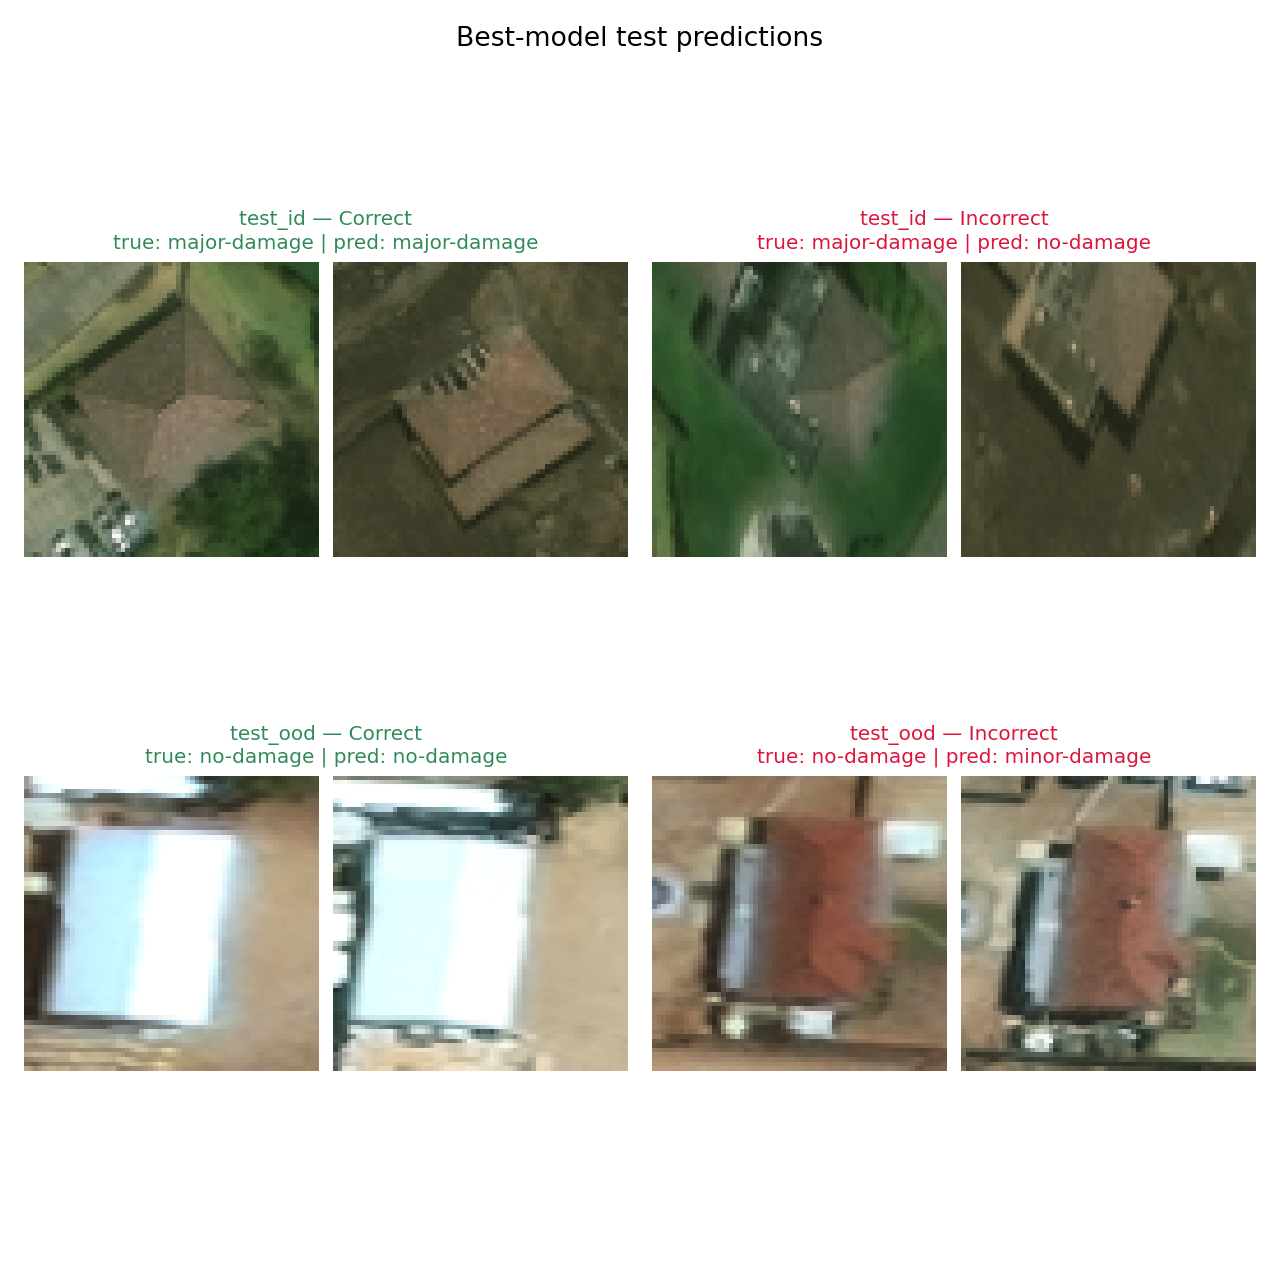
\includegraphics[width=\columnwidth]{figures/prediction_examples_pretrained.png}
\caption{Pretrained model: one correct and one incorrect prediction on \texttt{test\_id} and on
\texttt{test\_ood}, pre-disaster crop left and post-disaster crop right in each pair. The
\texttt{test\_ood} error is a truly undamaged building predicted \class{minor-damage}, the
over-flagging failure mode quantified above.}
\label{fig:predictions}
\end{figure}

The direction of the errors is equally consistent. For the from-scratch model, whose full confusion
matrices are available (Fig.~\ref{fig:confusion}), 81.1\% of out-of-domain errors
over-estimate severity against 18.9\% that under-estimate, and 35.9\% of truly undamaged wildfire
buildings (4,324 of 12,056) are flagged as damaged. The pretrained model shows the same failure mode
less severely: its \class{no-damage} recall of 0.805 on \texttt{test\_ood} corresponds to a
19.5\% false-alarm rate. Both confirm the prediction made from the exploratory analysis
before training.

\begin{figure*}[t]
\centering
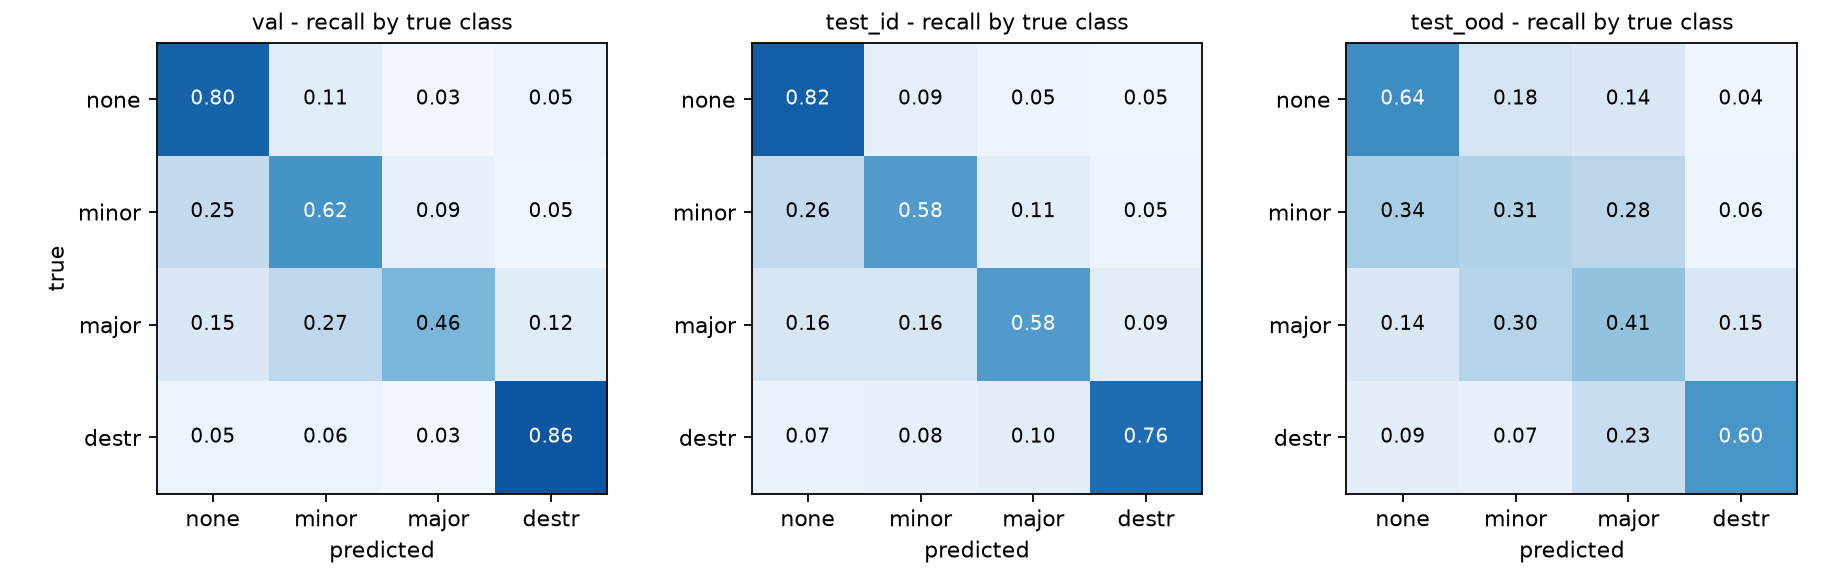
\includegraphics[width=0.85\textwidth]{figures/confusion_scratch.png}
\caption{Confusion matrices for the from-scratch model, normalised per true class (recall). The
\texttt{test\_ood} panel shows probability mass pushed off the diagonal in one direction, toward
greater severity, rather than scattered.}
\label{fig:confusion}
\end{figure*}

\subsection{Pretrained against from-scratch}
\label{sec:comparison}

This section addresses the project's second research question directly. Both models are trained on
identical patches, splits, class weights and evaluation code, and differ only in the encoder, which
isolates the effect of ImageNet pretraining from every other design choice. Pretraining outperforms
the from-scratch encoder on every split and every metric in Table~\ref{tab:main}, and the advantage
is largest where it matters most: on \texttt{test\_ood} it adds $+0.143$ accuracy, $+0.052$ macro-F1
(a 13.9\% relative gain over the from-scratch model's 0.377) and $+0.024$ ROC-AUC. The relative
macro-F1 drop from \texttt{test\_id} also shrinks, from 38.7\% for the from-scratch model to 33.9\%
for the pretrained one, so pretraining does not just raise the floor, it also makes the domain-shift
degradation proportionally smaller.

Per class, the clearest single difference is \class{destroyed}: 0.758 against 0.662 out of domain, and
0.687 against 0.563 in domain. The intermediate classes are not meaningfully distinguishable between
the two models, since both are far below usable precision, and at $n = 116$ and $n = 138$ the small
reversals observed there fall within noise. One caveat applies to this comparison: it is not a pure
pretraining ablation, since the pretrained encoder is also $8.4\times$ larger. A third run using the
same ResNet-18 architecture with random initialisation would separate the effect of pretraining from
the effect of capacity; we have not run it (Section~\ref{sec:limitations}).

% =====================================================================
\section{Discussion}
\label{sec:discussion}

\paragraph{Evidence for a calibration failure rather than a representation failure.} Four
observations support this reading of the 33.9\% macro-F1 drop.

\begin{enumerate}[leftmargin=*,itemsep=2pt,topsep=3pt,label=(\arabic*)]
\item \class{destroyed} scores higher out of domain than in it (0.758 against 0.687), and
\class{no-damage} precision is 0.966: the two classes that actually occur under wildfire are
recognised well.
\item The errors are directionally consistent, with 81.1\% over-estimating severity for the
model whose full confusion matrix is available. A consistent bias is the signature of a shifted
prior; a failure of the learned representation would instead be expected to produce diffuse,
symmetric confusion.
\item ROC-AUC, which does not depend on a decision threshold, holds at 0.814 against 0.908 in
domain: the ranking of predictions by severity survives, and it is the decision boundary that fails.
\item The collapse is arithmetically forced by the class-frequency shift. \class{minor} and
\class{major} make up 10.5\% and 8.6\% of training patches but only 0.79\% and 0.94\% of wildfire
patches. The pretrained model emits 2,814 intermediate predictions against 254 true cases, which caps
combined precision near 0.02 regardless of feature quality, and matches the 0.020 and 0.024 actually
measured.
\end{enumerate}

This distinction has direct operational consequences. A representation failure would mean the
approach cannot be deployed on a new disaster type at all. A calibration failure means the ranking of
predictions is usable and only the decision rule needs adjusting, a considerably more tractable
problem with an established remedy in prior correction~\cite{saerens}, which rescales class
posteriors by the ratio of target to source priors without retraining. A model of this kind deployed
on an unlabelled new disaster type would reliably separate destroyed from intact structures while
substantially over-reporting intermediate damage. For triage, i.e.\ prioritising where responders
look first, that failure mode is comparatively benign; for damage quantification, and
particularly for aid allocation, it is not.

% =====================================================================
\section{Impact and recovery analysis}
\label{sec:socio}

\subsection{Data and method}

To ask whether damage falls unequally across communities, we take the per-building WGS84 centroids in
the xBD labels, restrict to the ten US events for which census geography is available, and spatially
join them to 2020 TIGER census block groups. Each building contributes an ordinal damage score
(\class{no-damage} $= 0$ to \class{destroyed} $= 3$); the unit of analysis is the block-group mean.
Block groups with fewer than 20 buildings are dropped. That gives 185,045 buildings in
308 block groups, joined to American Community Survey covariates for 2017~\cite{acs}.

Two data-quality problems had to be handled first, and both are reported rather than absorbed
silently.

\paragraph{Census sentinel values.} The ACS extract encodes missing values as $-666666666$
rather than as nulls, and 17 of the 308 block groups carry one in median income, home value or year
built, which if left in place makes those coefficients meaningless. We drop them, leaving 291 block
groups.

\paragraph{Two unusable columns.} The poverty rate is empty for every block group, and the hazard
exposure proxy is identically zero because no fire-perimeter, storm-track or coastline layer was ever
joined. Both are dropped rather than reported as null effects.

The exposure control is therefore the built environment only (building density and median building
age), plus, in the strongest specification, event fixed effects. Event identity is the
sharpest exposure control this data supports: comparing two block groups inside the same disaster
holds the hazard roughly constant.

\subsection{Results}

\begin{table}[t]
\centering
\footnotesize
\caption{Standardised OLS coefficients on block-group mean damage score, $n = 291$. Each column adds
controls to the one before it: socioeconomic only, plus built environment, plus event fixed effects.}
\label{tab:socio}
\begin{tabular}{@{}lrrr@{}}
\toprule
& \textbf{naive} & \textbf{+ built} & \textbf{+ FE} \\
\midrule
Median income      & $+0.211^{**}$ & $+0.225^{***}$ & $+0.057$ \\
Median home value  & $-0.150^{**}$ & $-0.139^{*}$   & $-0.039$ \\
Renter share       & $+0.015$      & $+0.032$       & $-0.016$ \\
Building density   &               & $-0.085^{*}$   & $-0.103^{**}$ \\
Building age       &               & $-0.102^{*}$   & $-0.096^{*}$ \\
\midrule
$R^2$              & 0.045 & 0.072 & 0.225 \\
adjusted $R^2$     & 0.035 & 0.055 & 0.186 \\
\bottomrule
\end{tabular}
\vspace{2pt}
{\scriptsize $^{*}p<0.05$, $^{**}p<0.01$, $^{***}p<0.001$.}
\end{table}

Table~\ref{tab:socio} summarises the result. Regressed on socioeconomic variables alone, median
income carries a significant positive coefficient ($+0.211$, $p = 0.002$), and adding
built-environment controls strengthens it further ($+0.225$, $p = 0.0009$). Taken at face value,
this would indicate that richer block groups suffered more damage.

Adding event fixed effects destroys the effect. The income coefficient falls to $+0.057$ and is no
longer distinguishable from zero ($p = 0.44$), while $R^2$ more than triples, from 0.072 to 0.225.
Almost all of the apparent socioeconomic signal was between-event variation: \texttt{hurricane-\allowbreak harvey}
block groups have both high income (\$98k median) and high damage (mean score 0.88), while
\texttt{santa-\allowbreak rosa-wildfire} and \texttt{moore-tornado} have moderate income and low damage.

\begin{figure*}[t]
\centering
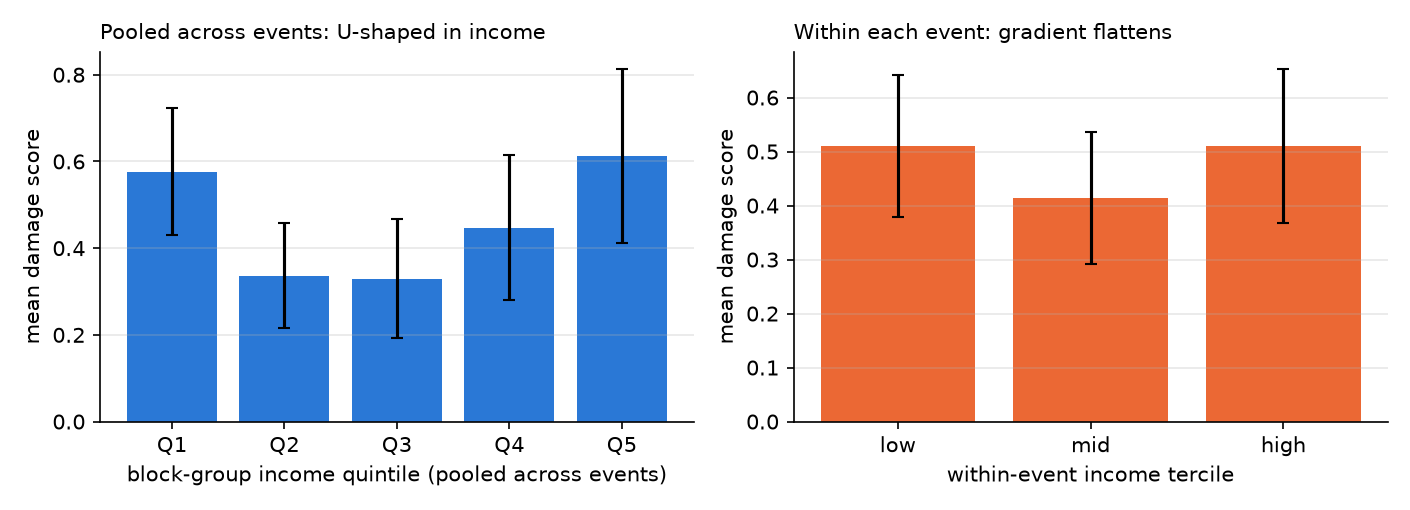
\includegraphics[width=0.85\textwidth]{figures/socio_income_gradient.png}
\caption{Left: pooling all ten events, mean damage score is U-shaped in income, highest in the
poorest and the richest quintiles and lowest in the middle. Right: once income terciles are computed
\emph{within} each event, the gradient flattens and the 95\% intervals overlap completely.}
\label{fig:socioincome}
\end{figure*}

Figure~\ref{fig:socioincome} shows the same thing without a model. Pooled across events the
relationship is U-shaped, not monotone: mean damage score is 0.58 in the poorest income quintile,
falls to 0.33 in the middle, and rises to 0.61 in the richest. That is what a mixture of two exposure
stories looks like, low-income tracts in tornado paths and high-income tracts in coastal and
wildland-urban-interface zones, rather than a single inequality gradient. Computing income terciles
within each event, over the six events with at least 15 block groups, flattens it to
0.50 / 0.43 / 0.50, and the per-event direction is inconsistent in sign: damage rises with income
across \texttt{hurricane-\allowbreak harvey} (0.77 to 1.01) and falls with it across \texttt{joplin-tornado}
(0.90 to 0.41).

\begin{figure}[t]
\centering
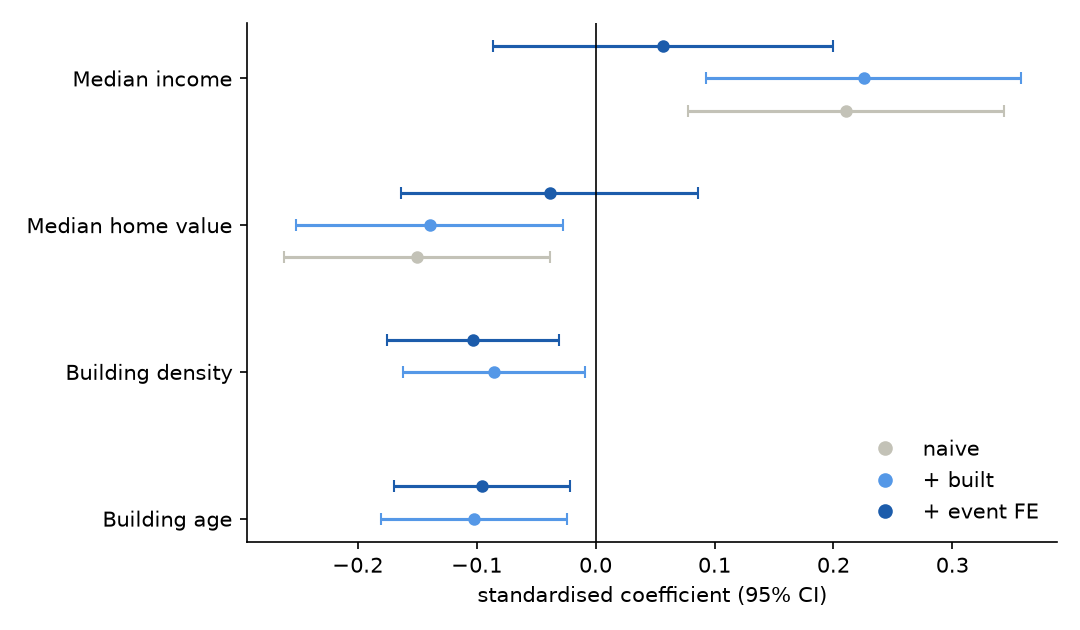
\includegraphics[width=\columnwidth]{figures/socio_coefficients.png}
\caption{Standardised coefficients with 95\% intervals across the three specifications. The two
socioeconomic effects shrink toward zero when event fixed effects enter; the two built-environment
effects do not.}
\label{fig:socioforest}
\end{figure}

What survives event fixed effects is the built environment: building density
($-0.103$, $p = 0.006$) and median building age ($-0.096$, $p = 0.012$) both remain significant and
barely move (Fig.~\ref{fig:socioforest}). Denser and older block groups record less damage on
average, which runs against the usual intuition that older housing is more vulnerable, and is most
plausibly a settlement-pattern effect: dense, older cores sit away from the coastal and interface
edges where these particular hazards concentrate.

\subsection{Pricing damage, and checking the price against real records}
\label{sec:socio-cost}

An ordinal damage class says nothing about the size of the loss it represents, and the project
specification asks about recovery as well as damage. To get at that, every building's damage
class is converted to a dollar figure using the HAZUS-MH per-damage-state loss ratios~\cite{hazus} ($0\%$ for
\class{no-damage}, $5\%$ \class{minor-damage}, $30\%$ \class{major-damage}, $100\%$
\class{destroyed}) applied to its block group's median home value. The rule is not disaster-specific:
a destroyed house costs its replacement value whichever hazard destroyed it. Over the 108,491
buildings inside the 291 analysis block groups this prices \$6.76B of modelled loss, with
wildfire alone accounting for 70\% of it (Californian home values are high and fire tends to destroy
outright), hurricane 22\%, tornado 7\%, and the single flood event under 1\%, so the dollar layer is
not simply a restatement of flood risk.

That price was checked against three independent, real-world records rather than taken on faith.
Against 6,525 National Flood Insurance Program settlements~\cite{openfema} inside the same block
groups, the modelled price lands at $0.32$--$0.85\times$ what the adjuster assessed on site: the
right order of magnitude, and consistently conservative. Against 9,395 CAL FIRE post-fire structure
inspections~\cite{calfire} for the three wildfire events, inspectors measured an average loss of
$91.4\%$ of a structure where the assumed ratios give $92.7\%$, within 1.3 points. And against
133,240 FEMA household loss verifications~\cite{openfema} spanning all ten events, the modelled price
runs well above FEMA's own figure, which is expected: FEMA's verified loss records the damage the aid
programme will pay for, a floor on the rebuild cost rather than an estimate of it.

\subsection{Recovery capacity is where the real inequality is}
\label{sec:socio-recovery}

Figure~\ref{fig:sociodollars} makes a point the regression above cannot. Physical damage is close to
flat across income ($10.6\%$ of building value lost in the poorest quintile against $11.7\%$ in the
richest, non-monotone), but the identical damage map priced in dollars is steep, rising from \$13k to
\$85k in modelled loss per building, a $\sim\!7\times$ gradient, simply because a home in a richer
block group costs more to begin with.

Who actually pays that bill tracks income even more sharply (Fig.~\ref{fig:sociowhopays}).
Restricting to the four water events, where the National Flood Insurance Program publishes a claim
for every settled property, claims filed per damaged building rise steeply with income (Spearman
$\rho = 0.63$): the poorest income quartile files a claim for $5\%$ of its damaged buildings against
$51\%$ in the richest. Splitting the repair bill three ways tells the same story: insurance covers
$24\%$ of the poorest quartile's modelled loss and FEMA grants another $16\%$, leaving $60\%$ covered
by nothing, while in the richest quartile insurance alone covers $66\%$ and only $33\%$ goes
uncovered.

FEMA's own applicant records extend this picture to every disaster type~\cite{openfema}. Among
115,463 owner-occupants who applied for federal aid, the insured share rises from $38\%$ in the
poorest household-income band to $95\%$ in the richest, and the gradient holds inside every disaster
type. This also corrects a flood-only impression: wildfire households are the best insured of the
four ($75\%$), and flood households the worst ($60\%$), because a standard homeowner policy covers
fire and wind while flood requires a separate NFIP policy.

\begin{figure*}[t]
\centering
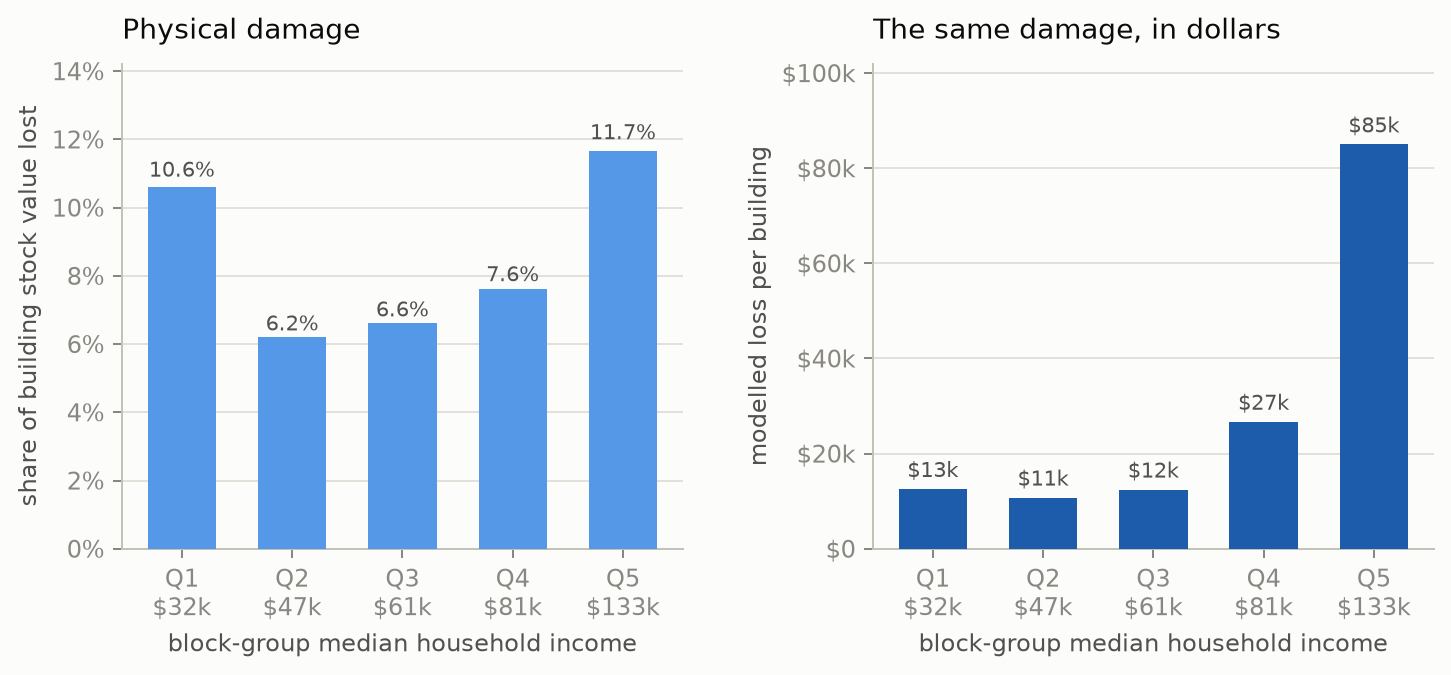
\includegraphics[width=0.85\textwidth]{figures/socio_damage_vs_dollars.png}
\caption{Left: share of building value lost, by block-group income quintile. Right: the identical
damage map, priced in dollars per building. Physical damage is roughly flat; the dollar figure is not.}
\label{fig:sociodollars}
\end{figure*}

\begin{figure*}[t]
\centering
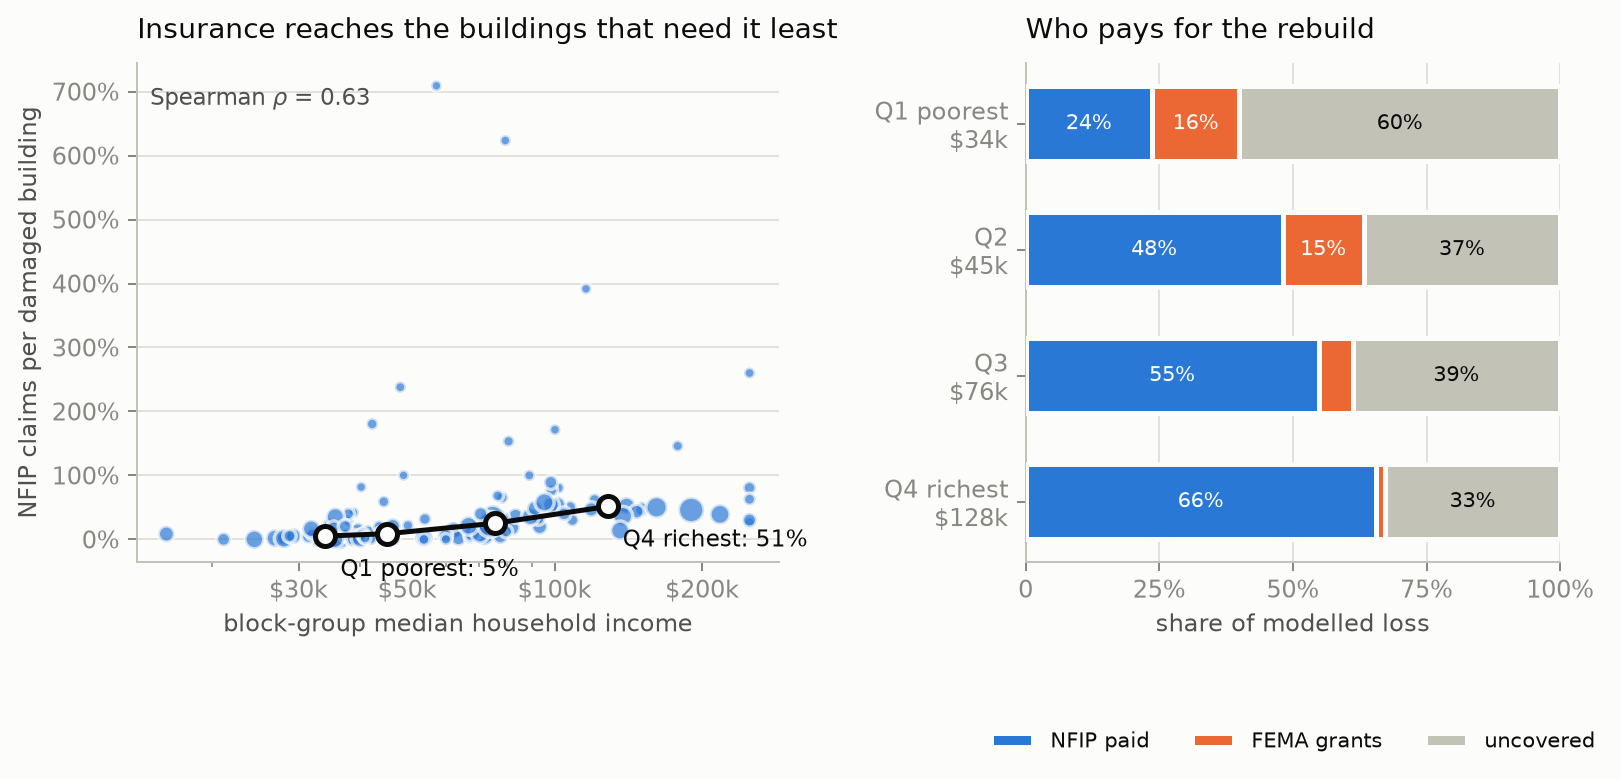
\includegraphics[width=0.85\textwidth]{figures/socio_who_pays.png}
\caption{Left: NFIP claims filed per damaged building against block-group income, the four water
events. Right: the repair bill split into what insurance paid, what FEMA paid, and what nobody paid,
by income quartile.}
\label{fig:sociowhopays}
\end{figure*}

\subsection{Auditing the predicted damage map}
\label{sec:socio-audit}

Every result up to this point uses xBD ground-truth labels, by design (Section~\ref{sec:socio-deploy}
explains why). The last question this data can answer directly is what changes if a relief programme
used the Part~2 models' predictions instead of verified labels. Joining the two models' output on
their held-out splits to the same census geography gives 12,438 buildings across seven events (three
hurricanes, one flood, three wildfires) and 122 block groups; tornado is absent from the audit for an
unrelated reason, since all three tornado events sit entirely inside the Part~2 training split and so
have no held-out predicted map.

We split a fixed \$1B relief budget by income tercile twice, once on the true damage map and once on
the pretrained model's predicted map, under two allocation rules (an equal payment per damaged
building, and a payment proportional to modelled dollar loss), and measure how many dollars land in a
different income tercile than the labels would send them. On the seen disaster types the predicted
map misdirects \$30--78M of every \$1B; on wildfire, the type the model never trained on, it is
\$112--200M (Fig.~\ref{fig:socioaudit}), and the direction is systematic rather than random:
consistent with the intermediate-class over-prediction documented in Section~\ref{sec:results}, the
model invents damage in mid-income block groups and withdraws funding from the high-income block
groups where the wildfires actually destroyed the housing. The predicted map also over-states the
total dollar loss on this sample by $19\%$. This is not a flaw specific to the pretrained model: the
from-scratch model's audit numbers are of the same order (\$37--81M seen, \$137--179M wildfire).

\begin{figure*}[t]
\centering
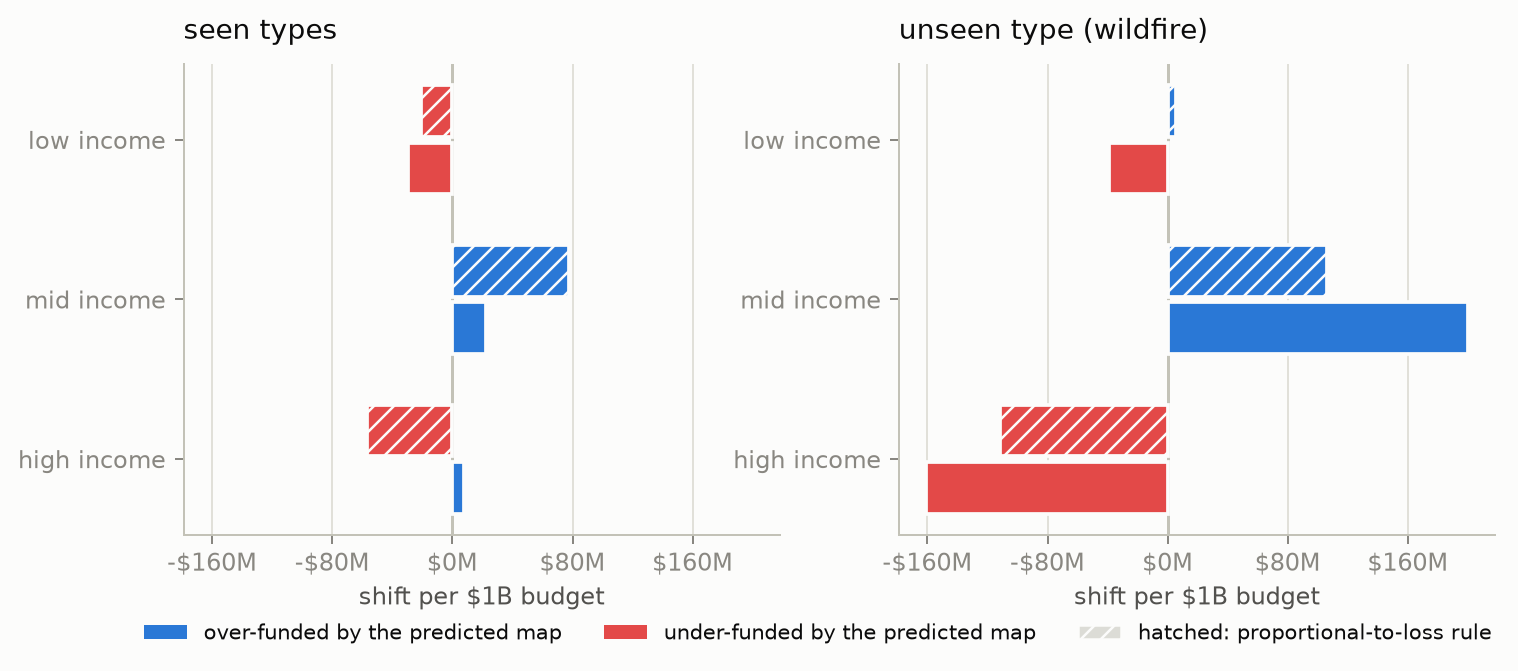
\includegraphics[width=0.85\textwidth]{figures/socio_model_misallocation.png}
\caption{Dollars per \$1B relief budget that land in a different income tercile under the predicted
map than under the true damage map, pretrained model. Blue over-funds a tercile, red under-funds it.
The wildfire panel is both larger and directionally consistent, unlike the seen-type panel.}
\label{fig:socioaudit}
\end{figure*}

\subsection{What this means for deployment}
\label{sec:socio-deploy}

Three cautions follow from this analysis, and they compound. First, the naive specification would
have supported a confident but incorrect policy claim: a pipeline that regressed damage on income and
reported the coefficient would have published a significant positive income effect that does not
survive the most basic exposure control available. The confounder here is not subtle; it is simply
which disaster struck which place.

Second, the recovery-capacity analysis in Section~\ref{sec:socio-recovery} shows an inequality the
damage regression cannot see: physical damage is close to flat across income, but dollar loss and the
capacity to cover it are not. A relief rule keyed to dollar damage, or to insurance status, is
regressive before any model is involved.

Third, Section~\ref{sec:results} showed that the model's errors are not random: it over-flags
intermediate damage at a rate that depends on the disaster type, and Section~\ref{sec:socio-audit}
shows what that costs in practice, moving real relief money along income lines and moving more of it
on the one disaster type the model has never seen. Rapid automated damage maps are useful for triage;
using them as evidence for aid allocation without verified labels risks more than generic error, it
risks a specific, income-correlated error, in the direction the model already over-predicts.

% =====================================================================
\section{Limitations}
\label{sec:limitations}

\begin{itemize}[leftmargin=*,itemsep=2pt,topsep=3pt]
\item \textbf{Thin out-of-domain support.} \class{minor} and \class{major} rest on 116 and 138 true
examples in \texttt{test\_ood}. These two classes drive the macro-F1 story, so their per-class figures
carry wide uncertainty.
\item \textbf{Annotator selection.} Every number is measured on buildings annotators were able
to assess, since \class{un-classified} polygons are excluded, so true zero-shot difficulty is
somewhat higher than reported.
\item \textbf{Partial checks and sampling.} The
duplicate test covers 400 of 11,034 scenes and model
results use a stratified sample of 1,698 scenes (the
acquisition-geometry confound is discussed in
Section 3.4.
\item \textbf{Not a pure pretraining ablation}, since the encoders differ in initialisation and in
size (11.57M against 1.37M parameters); and model selection uses \texttt{val}, which is
in-distribution, because selecting on the out-of-domain set would leak the test set.
\item \textbf{Ecological inference in Part 3.} Block-group averages cannot support claims about
individual households, no true hazard-exposure layer was available, and ten events is a small basis
for fixed effects.
\item \textbf{Recovery-analysis assumptions.} One median home value stands in for every building in
a block group, and four HAZUS loss ratios stand in for a continuous damage distribution. Tornado has
no inspection dataset comparable to CAL~FIRE's, so its loss ratios rest on the HAZUS assumption
alone. Insurance take-up from FEMA records describes owner-occupants who applied for aid, not the
general population, and the predicted-damage audit covers seven of the ten events because the three
tornado events never appear in a held-out split.
\end{itemize}

% =====================================================================
\section{Conclusions and next steps}

This project set out to answer two questions: whether building-damage classification transfers to a
disaster type withheld from training, and whether ImageNet pretraining improves that transfer
relative to a comparable encoder trained from scratch. On the first question, a siamese
change-detection CNN trained on 14 non-fire disasters and evaluated zero-shot on five wildfire events
loses a third of its macro-F1, but the loss is confined to the two damage classes that barely exist
under wildfire, while destroyed-versus-intact discrimination improves out of domain. On the
second, ImageNet pretraining outperforms the from-scratch encoder on every split and every metric,
with the largest margin precisely on the wildfire set. A supplementary impact analysis finds that raw
damage is not distributed along an income gradient once the disaster event itself is controlled for,
but that finding does not extend to recovery: priced in dollars, and measured against real insurance
and federal-aid records, the same damage falls on households with sharply unequal capacity to pay for
it, and auditing the Part~2 models' own predictions shows that an automated relief rule would move
real money along income lines, more so on the disaster type the models never trained on. Outstanding
work, in priority order:

\begin{enumerate}[leftmargin=*,itemsep=2pt,topsep=3pt]
\item \textbf{Test the calibration hypothesis directly.} Apply prior correction~\cite{saerens} to the
out-of-domain predictions of both models and measure how much of the macro-F1 gap closes without
retraining. If most of it closes, that is the strongest result the project can report.
\item \textbf{Few-shot ablation}: add 1 to 5\% of wildfire scenes to training and re-measure the gap.
\item \textbf{Randomly initialised ResNet-18} as a third run, to separate pretraining from capacity.
\item \textbf{Real hazard-exposure layers} for Part 3, in place of the event-fixed-effects proxy, and
a tornado inspection dataset comparable to CAL~FIRE's to remove the last HAZUS-only loss ratio.
\end{enumerate}

\paragraph{Reproducibility.} Every figure, table and number in this report is generated from a CSV
artefact written by the notebooks and scripts in the repository; nothing is hand-computed. Seed 42
throughout. Environment setup, data sources, and a map from each notebook to the results and figures
it produces are documented in the repository \texttt{README.md}.

% =====================================================================
\begin{thebibliography}{9}
\small

\bibitem{xbd}
R.~Gupta \emph{et al.},
``xBD: A Dataset for Assessing Building Damage from Satellite Imagery,''
\emph{arXiv:1911.09296}, 2019.

\bibitem{fusion}
E.~Weber and H.~Kan\'e,
``Building Disaster Damage Assessment in Satellite Imagery with Multi-Temporal Fusion,''
\emph{arXiv:2004.05525}, 2020.

\bibitem{resnet}
K.~He, X.~Zhang, S.~Ren and J.~Sun,
``Deep Residual Learning for Image Recognition,'' \emph{CVPR}, 2016.

\bibitem{imagenet}
J.~Deng \emph{et al.},
``ImageNet: A Large-Scale Hierarchical Image Database,'' \emph{CVPR}, 2009.

\bibitem{lpft}
A.~Kumar, A.~Raghunathan, R.~Jones, T.~Ma and P.~Liang,
``Fine-Tuning can Distort Pretrained Features and Underperform Out-of-Distribution,''
\emph{ICLR}, 2022.

\bibitem{saerens}
M.~Saerens, P.~Latinne and C.~Decaestecker,
``Adjusting the Outputs of a Classifier to New a Priori Probabilities,''
\emph{Neural Computation}, 14(1):21-41, 2002.

\bibitem{pytorch}
A.~Paszke \emph{et al.},
``PyTorch: An Imperative Style, High-Performance Deep Learning Library,'' \emph{NeurIPS}, 2019.

\bibitem{acs}
U.S. Census Bureau, American Community Survey 5-Year Estimates (2017) and TIGER/Line block-group
boundaries (2020).

\bibitem{xview2}
xView2 Challenge, \url{https://xview2.org}.

\bibitem{hazus}
Federal Emergency Management Agency, \emph{Hazus -- Multi-Hazard Loss Estimation Methodology
(Hazus-MH)}, Technical Manual, \url{https://www.fema.gov/flood-maps/tools-resources/flood-map-products/hazus}.

\bibitem{openfema}
Federal Emergency Management Agency, OpenFEMA API: \emph{FIMA NFIP Redacted Claims},
\emph{Individuals and Households Program Valid Registrations}, and disaster declaration summaries,
\url{https://www.fema.gov/about/openfema/data-sets}.

\bibitem{calfire}
California Department of Forestry and Fire Protection (CAL FIRE), \emph{Damage Inspection (DINS)
Data}, \url{https://www.fire.ca.gov/programs/fire-prevention/wildfire-preparedness/damage-inspection-dins-data}.

\end{thebibliography}

\end{document}
